\documentclass[english,xcolor=dvipsnames]{beamer}
\usepackage[autolinebreaks,useliterate]{mcode}
\usepackage[orientation=landscape,size=custom,width=16,height=9,scale=0.48,debug]{beamerposter}
\usepackage[T1]{fontenc}
\usepackage[latin9]{inputenc}
\usepackage{amsthm}
\usepackage{amsmath}
\usepackage{amssymb}
\usepackage{bookmark}
\usepackage{graphics,graphicx}
\usepackage{pstricks,pst-node,pst-tree}
\usefonttheme{serif}
\usepackage{palatino}
\usepackage{tikz}
\usetikzlibrary{shapes,arrows}
\usetikzlibrary{positioning}
%\usepackage[margin=.5cm]{geometry}

\definecolor{dgreen}{rgb}{0.,0.6,0.}
\definecolor{forest}{RGB}{34.,139.,34.}
\definecolor{byublue}{RGB}{0.,30.,76.}
\definecolor{dukeblue}{RGB}{0.,0.,156.}
%\usetheme{Ilmenau}
\usetheme{Warsaw}
\usecolortheme[named=dukeblue]{structure}
%\usecolortheme[named=RawSienna]{structure}
%\usecolortheme[named=byublue]{structure}
\setbeamertemplate{navigation symbols}{}
\setbeamertemplate{footline}{}
\setbeamercovered{transparent}

\newcommand{\be}{\begin{enumerate}}
\newcommand{\ee}{\end{enumerate}}
\newcommand{\bq}{\begin{quote}}
\newcommand{\eq}{\end{quote}}
\newcommand{\bd}{\begin{description}}
\newcommand{\ed}{\end{description}}
\newcommand{\bi}{\begin{itemize}}
\newcommand{\ei}{\end{itemize}}

\title[]{Multinomial Choice}
\author{Tyler Ransom}
\institute{Duke University}
\date{\today}

\begin{document}

\begin{frame}
   \titlepage
\end{frame}

\begin{frame}
\frametitle{Multinomial Choice}
   \bi 
   \item In Applied Micro, a common and straightforward way to model an agent's behavior is through a discrete choice model
   \item Agent faces $J$ mutually-exclusive choices
      \bi 
      \item E.g. get to work via bicycle, bus, car, or other
      \ei
   \item We want to see how the agent's dependent variable (taking on values $1, 2, \ldots, J$) varies with some covariates ($X$)
   \ei
\end{frame}

\begin{frame}
\frametitle{Binary logit}
   \bi 
   \item Recall the choice probabilities from the binary logit model, where $y = X\beta + \varepsilon$ and $y \in \{0,1\}$:\\ $P_{1} = \frac{\exp(X\beta)}{1+\exp(X\beta)}$\\ $P_{0} = 1-P_{1} = \frac{1}{1+\exp(X\beta)}$
   \item $\beta_{0}$ is normalized to $0$ in this model to identify $\beta$
   \ei
\end{frame}

\begin{frame}
\frametitle{Multinomial Logit}
   \bi 
   \item Given $y=X\beta + \varepsilon$, the probability that choice $j$ is selected is $P_{j} = \frac{\exp(X\beta_{j})}{\sum_{k} \exp(X\beta_{k})}$
   \item Like in the binary case, normalize one of the $\beta_{j}$ to $0$ (for identification)
   \item Then the choice probability formula becomes $P_{j} = \frac{\exp(X\beta_{j})}{1+\sum_{h}\exp(X\beta_{h})}$
   \item Multinomial logit just adds more terms to the denominator and has $J$ separate probability formulas (instead of two)
   \ei
\end{frame}

\begin{frame}
\frametitle{Applications of Multinomial Choice}
IO
      \bi 
      \item Consumer decides which brand of a product to purchase (Demand estimation)
      \item Firm decides whether or not to enter a market (entry game)
      \ei
Labor
      \bi 
      \item Individual determines whether to attend college, enter the workforce, or exit the labor force
      \item Individual chooses which occupation (or industry) to work in
      \ei
Health
      \bi 
      \item Worker chooses a health insurance plan from a menu
      \item Patient decides which hospital to attend for treatments
      \ei
Urban/Environmental
      \bi 
      \item Individual chooses which city (or neighborhood within a city) to live in
      \item Parents choose which school to enroll children in
      \ei
\end{frame}

\begin{frame}
\frametitle{Random Utility Models}
   \bi 
   \item Useful to think of a multinomial choice model as a utility model
   \item Each agent gets utility from each of the choices, but the researcher only observes the choice of the agent (not the utility)
   \item Researcher assumes that utility-maximizing choice is the one observed
   \item This class of models is referred to as random utility models (``random'' because the choice has a random aspect to it---$\varepsilon$---and ``utility'' because utility is being modeled)
   \ei
\end{frame}

\begin{frame}
\frametitle{Identification in Random Utility Models}
   \bi 
   \item Normalizations:
   \item Scale: In the random utility model, one can multiply each of the alternatives by a constant without affecting which alternative is the $\max$
   \item Level: Similarly, one can add a positive constant to all alternatives without affecting the $\arg \max$
   \item In practice, scale is set by normalizing the variance of $\varepsilon_{ij}$ and level is set by normalizing one of the $\beta_{j}$'s to be zero
   \ei
\end{frame}

\begin{frame}
\frametitle{Distribution of Error Term}
   \bi 
   \item Our random utility model is $u_{ij} = x_{i}\beta_{j} + \varepsilon_{ij}$ where $i$ indexes individuals and $j$ indexes choices
   \item For a multinomial logit, assume $\varepsilon_{ij}$ is iid standard Type I Extreme Value [$F(x) = e^{-e^{-x}}$]
   \item Normalize the variance of $\varepsilon_{ij}$ to $\pi^{2}/6$
   \item The familiar logistic distribution is nothing more than a difference in two T1EV variables with the appropriate normalizations already imposed
   \item This yields the choice probability formulas described earlier
   \item Standard T1EV (Gumbel) distribution looks similar to a normal, but with fatter tails
   \ei
\end{frame}

\begin{frame}
\frametitle{Distribution of Error Term}
   \bi 
   \item If errors are normal, assume $\varepsilon_{ij} \sim N\left(0,\Omega\right)$
   \item Where $\Omega$ is some covariance matrix
   \item Note: can't estimate all covariance matrix elements, because scale needs to be set
   \item No one way to normalize this, but most common way is to set one of the variances to 1
   \ei
\end{frame}

\begin{frame}
\frametitle{Logit vs. Probit}
\begin{figure}
	\caption{Logit vs. Probit PDF}
	\centering
		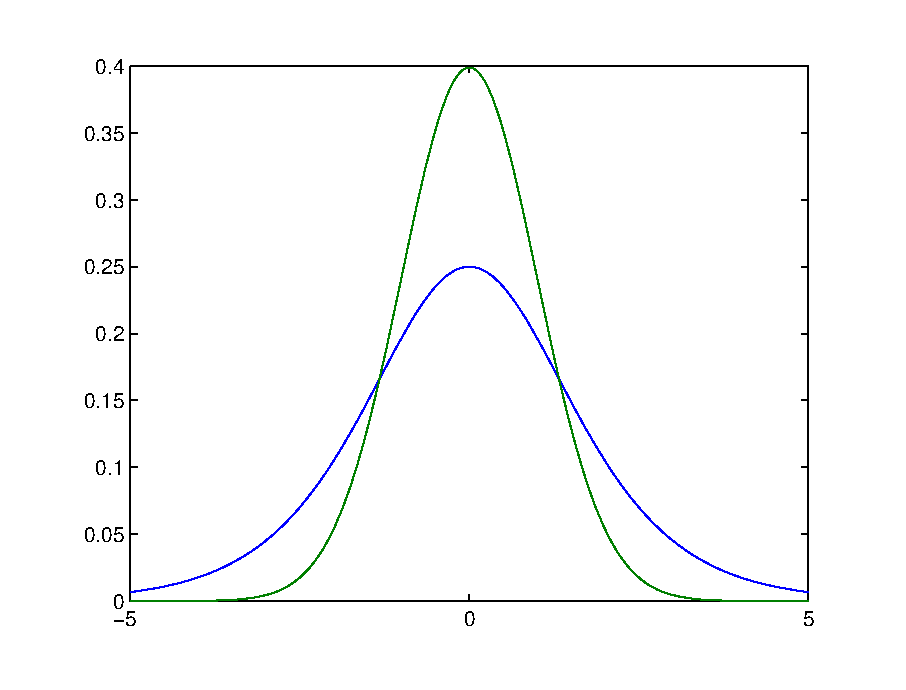
\includegraphics[scale=0.40]{EVvsNormalpdf.eps}\\
	\footnotesize{Note: Logit in blue; Normal in green}
	\label{fig:EVvsNormalpdf}
\end{figure}
\end{frame}


\begin{frame}
\frametitle{Independence of Irrelevant Alternatives (IIA)}
   \bi 
   \item The major drawback of the logit model is its vulnerability to the IIA assumption, which imposes too many restrictions on substitution patterns (see next slide)
   \item Mathematically, this is manifest by comparing the ratio of two $P_{ij}$'s:
   \item $P_{i1} = \exp(x_{i}\beta_{1})/(\textrm{denominator})$
   \item $P_{i3} = \exp(x_{i}\beta_{3})/(\textrm{denominator})$
   \item $\frac{P_{i1}}{P_{i3}} = \exp(x_{i}\beta_{1})/\exp(x_{i}\beta_{3}) = \exp(x_{i}(\beta_{1}-\beta_{3}))$
   \item So the ratio of the probabilities is the same regardless of how many other choices there are
   \ei
\end{frame}

\begin{frame}
\frametitle{Red Bus / Blue Bus Example}
   \bi 
   \item McFadden (1974) provides a famous example of the drawbacks to the IIA assumption
   \item Suppose a commuter is initially faced with two options: red bus and car, and that each choice probability is 1/2
   \item Now suppose a new choice is introduced: blue bus
   \item The IIA assumption requires that the new choice probabilities are 1/3 for each choice
   \item But given that commuters don't care what color the bus is, the actual change in probabilities is unlikely to be so drastic
   \ei
\end{frame}

\begin{frame}
\frametitle{Getting around IIA}
   \bi 
   \item Nested Logit
      \bi 
      \item Allows correlation among alternatives within a ``nest'' of choices
      \ei
   \item Other GEV forms
      \bi 
      \item Assume $\varepsilon_{ij}$ is distributed Generalized Extreme Value (instead of iid Type 1 EV)
      \ei
   \item Note: GEV forms still have closed-form choice probabilities, which is a huge advantage
   \item You'll cover these topics in more detail in Peter Arcidiacono's 2nd-year class
   \ei
\end{frame}

\begin{frame}
\frametitle{Choice of Error: Logit vs. Probit}
   \bi 
   \item Logit Pros:
      \bi 
      \item Closed-form choice probabilities
      \ei
   \item Logit Cons:
      \bi 
      \item Have to have iid assumption
      \item This leads to the IIA problem
      \ei
   \item Probit Pros:
      \bi 
      \item Flexibly accommodates covariance among choice errors, so no issues with IIA
      \ei
   \item Probit Cons:
      \bi 
      \item Choice probabilities don't have closed form
      \item Requires computation (and simulation) of a $J-1$ dimensional integral
      \ei
   \ei
\end{frame}

\begin{frame}
\frametitle{Logit Drawbacks}
   \bi 
   \item Three main drawbacks to the logit
      \bi 
      \item It can't handle individual-specific betas
      \item Restrictive substitution patterns (IIA)
      \item Can't handle temporally-correlated $\varepsilon_{ij}$'s in panel data very well
      \ei
   \item Normal can get around all three of these, but at significant computational cost
   \item Nested Logit and other GEV models can only correct for the IIA assumption
   \item At the end of the day, most researchers still use logit because its computational ease is worth more than its drawbacks
   \ei
\end{frame}
\end{document}
